\chapter{Evaluation}

\begin{enumerate}
    \item evaluates your work (both in absolute terms, and compared to other solutions)
    \item objectives
    \item explain what was evaluated or validated
    \item experimental setup - detail how you evaluated and validated your work.
    \item present your results clearly and objectively, without interpretation - ideally with graphs (data)
    \item explain your results - ideally with explanatory text (analysis) to both explain the meaning of these results, and provide the reasons for why these particular results were obtained
    \item critically analyse your results. Identify the contents in which your results are relevant and any threats are to the validity of your results. Show how well you have answered the research question.
    \item Critically analyse your results with respect to the "Related Work" presented earlier.
\end{enumerate}

In this section we explain the experimental setup, experimental results and discuss the results of the several experiment conducted in detail. 

\section{Evaluation Metrics}
In this section we explain the evaluation metrics used in the experiments. In the experiments we use commonly used evaluation metrics like, sensitivity, specificity, accuracy, roc curve. Table~\ref{tab:configs} shows the possible outcomes of the experiments conducted. True positives are the number of truly detected subjects as abnormal, false negatives are the abnormal subjects but detected as normal by the test. Similarly true negative is number of truly detected subjects as being normal and false positives are subjects that are normal but classified as abnormal by the tests. Notice that depending on the experiments abnormal either means having diabetic retinopathy or having mocelar edema. Definitions of the evaluation metrics are as follows: 

\begin{align*}
    \textit{sensitivity} &= \frac{\textit{TP}}{\textit{TP} + \textit{FN}}
    &
    \textit{specificity} &= \frac{\textit{TN}}{\textit{TN} + \textit{FP}}
\end{align*}

\begin{align*}
    \textit{accuracy} &= \frac{\textit{TP} + \textit{TN}}{\textit{TP} + \textit{FP} + \textit{TN} + \textit{FN}}
\end{align*}

\begin{table}[t]
\centering
\caption{Test subject definitions} 
\label{tab:configs}
\begin{tabular}{|c|c|c|c|} \hline
     & Abnormal & Normal & Total  \\ \hline
     Abnormal& True Positive (TP) & False Positive (FP) & TP + FP \\ \hline
     Normal & False Negative (FN) & True Negative (TN) & TN + FN \\ \hline
     Total & TP + FN &  FP + TN & TP + FN + FP + TN \\ \hline
\end{tabular}
\end{table}

\subsection{Receiver operating characteristic (ROC)}
Another evaluation metric commonly used for diabetic retinopathy research is ROC. ROC is grahical representation of the fraction of TP  vs. FP. TP rate is also known as sensitivity, and FP rate is 1 minus the specificity. 


\section{Experiments with Messidor Dataset}
We run all the experiments in this section by using k-fold cross validation with the settings of k=6. We first shuffle the dataset and split the dataset into 6 folds. Each time we use 80\% of the data as training data and 20\% as test data. We run the following experiments.
\subsection{DR vs NonDR}
Binary classification.
\subsection{DR degree prediction}
This is 4 class prediciton.
\subsection{MA vs NonMA}
\section{Experiments by using other datasets}
In this section we train a convolutional neural network model by using all of the Messidor dataset as training data. 
\subsection{Stare Dataset Experiments}
In this part, we show the results of the experiments run with using Messidor dataset as traiing data and Stare dataset as test data. 93 DR and 36 NONDR data. 

\begin{figure}[b]
\centering
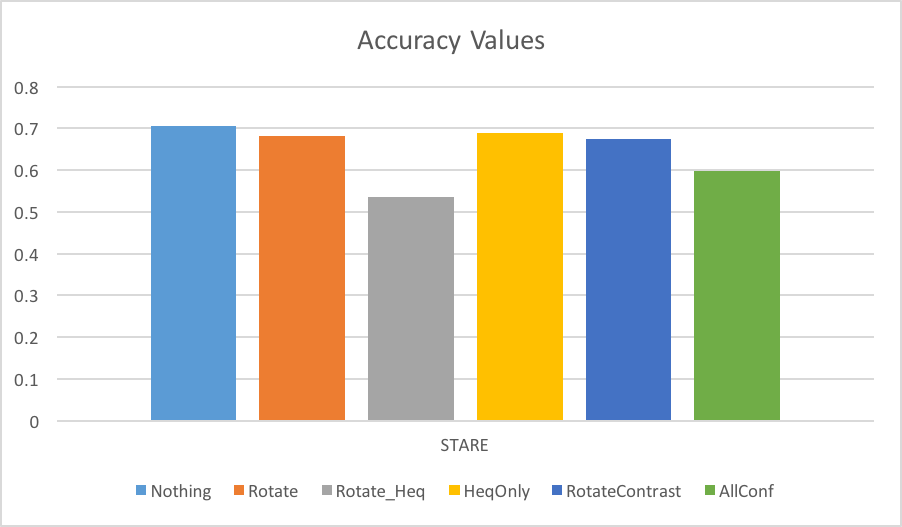
\includegraphics[width=0.8\textwidth]{Figures/stare.png}
\caption{Accuracy results for Stare dataset with different preprocessing steps}
\label{delta}
\end{figure}
